

\begin{figure}[!t]
\centering
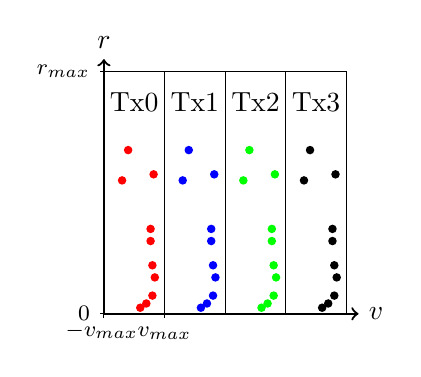
\begin{tikzpicture}[scale=0.77]
% Draw axes
%	\node[above] at (2,4) {SISO};
%
%    \draw [<->,thick] (0,4.2) node (yaxis) [above] {$r$}
%        |- (4.2,0) node (xaxis) [right] {$v$};
%    \draw[draw = black] (0pt,2pt) -- (0pt,-2pt) node[below] {\footnotesize $-v_\text{max}$};
%    \draw[draw = black] (2,2pt) -- (2,-2pt) node[below] {\footnotesize $0$};
%    \draw[draw = black] (4,2pt) -- (4,-2pt) node[below] {\footnotesize $v_\text{max}$};
%    \draw[draw = black] (2pt,0) -- (-2pt,0) node[left] {\footnotesize $0$};
%    \draw[draw = black] (2pt,4) -- (-2pt,4) node[left] {\footnotesize $r_\text{max}$};
%% Draw rectangles
%    \draw[draw=black] (0,0) rectangle ++(4,4);
%% Draw Objects
%    \fill[red] (1.8,2.2) circle (2pt);
%    \fill[red] (1.9,2.7) circle (2pt);
%    \fill[red] (2.1,0.1) circle (2pt);
%    \fill[red] (2.2,0.17) circle (2pt);
%    \fill[red] (2.3,0.3) circle (2pt);
%    \fill[red] (2.34,0.6) circle (2pt);
%    \fill[red] (2.3,0.8) circle (2pt);
%    \fill[red] (2.27,1.2) circle (2pt);
%    \fill[red] (2.27,1.4) circle (2pt);
%    \fill[red] (2.32,2.3) circle (2pt);
%    %
%\node[ align = center, rotate = 85] at (0.75,2) {\small Usually free of objects};
%\node[ align = center, rotate = 85] at (3.25,2) {\small Usually free of objects};
%\draw[draw = none, fill=gray, fill opacity=0.2, draw opacity=0] (0,0) rectangle ++(1.5,4);
%\draw[draw = none, fill=gray, fill opacity=0.2, draw opacity=0] (2.5,0) rectangle ++(1.5,4);
    % 
    \begin{scope}[shift={(5.3,0)}]
   % \node[above] at (2,4) {DDM};
    % Draw axes
    \draw [<->,thick] (0,4.2) node (yaxis) [above] {$r$}
        |- (4.2,0) node (xaxis) [right] {$v$};
%    \draw[draw = black] (0pt,2pt) -- (0pt,-2pt) node[below] {\footnotesize $-v_\text{max}$};
%    \draw[draw = black] (2,2pt) -- (2,-2pt) node[below] {\footnotesize $0$};
%    \draw[draw = black] (4,2pt) -- (4,-2pt) node[below] {\footnotesize $v_\text{max}$};
    \draw[draw = black] (2pt,0) -- (-2pt,0) node[left] {\footnotesize $0$};
    \draw[draw = black] (2pt,4) -- (-2pt,4) node[left] {\footnotesize $r_\text{max}$};

% Draw rectangles
    \draw[draw=black] (0,0) rectangle ++(1,4);
    \draw[draw=black] (1,0) rectangle ++(1,4);
    \draw[draw=black] (2,0) rectangle ++(1,4);
    \draw[draw=black] (3,0) rectangle ++(1,4);
% Draw Tx indication
    \node[align = center] at (0.5,3.5) {Tx0};
    \node[align = center] at (1.5,3.5) {Tx1};
    \node[align = center] at (2.5,3.5) {Tx2};
    \node[align = center] at (3.5,3.5) {Tx3};
% Draw Objects
	\fill[red] (1.8-1.5,2.2) circle (2pt);
    \fill[red] (1.9-1.5,2.7) circle (2pt);
    \fill[red] (2.1-1.5,0.1) circle (2pt);
    \fill[red] (2.2-1.5,0.17) circle (2pt);
    \fill[red] (2.3-1.5,0.3) circle (2pt);
    \fill[red] (2.34-1.5,0.6) circle (2pt);
    \fill[red] (2.3-1.5,0.8) circle (2pt);
    \fill[red] (2.27-1.5,1.2) circle (2pt);
    \fill[red] (2.27-1.5,1.4) circle (2pt);
    \fill[red] (2.32-1.5,2.3) circle (2pt);
    
    \fill[blue] (1.8-0.5,2.2) circle (2pt);
    \fill[blue] (1.9-0.5,2.7) circle (2pt);
    \fill[blue] (2.1-0.5,0.1) circle (2pt);
    \fill[blue] (2.2-0.5,0.17) circle (2pt);
    \fill[blue] (2.3-0.5,0.3) circle (2pt);
    \fill[blue] (2.34-0.5,0.6) circle (2pt);
    \fill[blue] (2.3-0.5,0.8) circle (2pt);
    \fill[blue] (2.27-0.5,1.2) circle (2pt);
    \fill[blue] (2.27-0.5,1.4) circle (2pt);
    \fill[blue] (2.32-0.5,2.3) circle (2pt);
    
	\fill[green] (1.8+0.5,2.2) circle (2pt);
    \fill[green] (1.9+0.5,2.7) circle (2pt);
    \fill[green] (2.1+0.5,0.1) circle (2pt);
    \fill[green] (2.2+0.5,0.17) circle (2pt);
    \fill[green] (2.3+0.5,0.3) circle (2pt);
    \fill[green] (2.34+0.5,0.6) circle (2pt);
    \fill[green] (2.3+0.5,0.8) circle (2pt);
    \fill[green] (2.27+0.5,1.2) circle (2pt);
    \fill[green] (2.27+0.5,1.4) circle (2pt);
    \fill[green] (2.32+0.5,2.3) circle (2pt);

    \fill[black] (1.8+1.5,2.2) circle (2pt);
    \fill[black] (1.9+1.5,2.7) circle (2pt);
    \fill[black] (2.1+1.5,0.1) circle (2pt);
    \fill[black] (2.2+1.5,0.17) circle (2pt);
    \fill[black] (2.3+1.5,0.3) circle (2pt);
    \fill[black] (2.34+1.5,0.6) circle (2pt);
    \fill[black] (2.3+1.5,0.8) circle (2pt);
    \fill[black] (2.27+1.5,1.2) circle (2pt);
    \fill[black] (2.27+1.5,1.4) circle (2pt);
    \fill[black] (2.32+1.5,2.3) circle (2pt);
    
    \draw[draw = black] (1,2pt) -- (1,-2pt);% node[below] {\footnotesize $v_\text{max}$};
    \draw[draw = black] (0,2pt) -- (0,-2pt);% node[below] {\footnotesize $-v_\text{max}$};
    
    \node at (-1pt,-8pt) {\footnotesize $-v_\text{max}$};
	\node at (1,-9pt) {\footnotesize $v_\text{max}$};
	
	
  \end{scope}
\end{tikzpicture}
\caption{ Sketch of an RDM for DDM with $N_\text{Tx}=4$ transmit antennas. Every real object results in $N_\text{Tx}$ peaks in the RDM, each one associated with one Tx antenna. }
\label{fig_DDM_DDM}
\end{figure}